\documentclass[12pt,a4paper]{article}
\usepackage[UTF8]{ctex}
\usepackage{amsmath,amssymb}
\usepackage{listings}
\usepackage{xcolor}
\usepackage{hyperref}
\usepackage{geometry}
\usepackage{graphicx}
\geometry{margin=2.5cm}

\lstdefinestyle{python}{
  language=Python,
  basicstyle=\ttfamily\small,
  keywordstyle=\color{blue}\bfseries,
  commentstyle=\color{gray},
  stringstyle=\color{red},
  showstringspaces=false,
  breaklines=true,
  frame=single,
  backgroundcolor=\color{gray!10}
}

\title{Hadamard Test / Hadamard 测试}
\author{QuoNic}
\date{}

\begin{document}
\maketitle

\begin{center}
\textbf{Algorithms / 算法} | 难度：中级 | 预计时间：10 分钟
\end{center}

\tableofcontents
\newpage

\section{为什么需要？}

Hadamard 测试用于估计 $\langle\psi|U|\psi\rangle$，是量子算法的基本工具。

\subsection{经典局限}
\b\begin{itemize}
  \item 经典方法需要知道 $|\psi\rangle$ 的具体形式
  \item 对于未知量子态，经典方法效率低
\end{itemize}

\subsection{量子优势}
\b\begin{itemize}
  \item Hadamard 测试只需要 1 个辅助量子比特
  \item 可以高效估计 $\text{Re}\langle\psi|U|\psi\rangle$
  \item 是量子算法设计的基本工具
\end{itemize}

\subsection{实际应用}
\b\begin{itemize}
  \item 量子算法设计
  \item 量子态验证
  \item 量子化学（能量估计）
\end{itemize}

\section{快速上手}

\begin{lstlisting}[style=python]
from quonic.algorithms import hadamard_test

# Estimate <psi|U|psi>
result = hadamard_test(state="0", gate="X")
print(f"Re(<psi|U|psi>): {result.expectation:.3f}")
\end{lstlisting}

\textbf{预期输出}：
\begin{verbatim}
Re(<psi|U|psi>): 0.000
\end{verbatim}

\section{原理详解}

\subsection{电路图}

\begin{center}
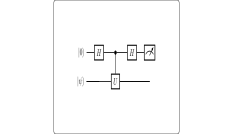
\includegraphics[width=0.6\textwidth]{../../images/hadamard_test_circuit.svg}
\end{center}

\subsection{数学推导}

Hadamard 测试估计：
\begin{equation}
P(|0\rangle) = \frac{1 + \text{Re}\langle\psi|U|\psi\rangle}{2}
\end{equation}

因此：
\begin{equation}
\text{Re}\langle\psi|U|\psi\rangle = 2P(|0\rangle) - 1
\end{equation}

\subsection{几何解释}

Hadamard 测试通过受控 $U$ 门和 Hadamard 门，将 $\text{Re}\langle\psi|U|\psi\rangle$ 编码到辅助量子比特的测量概率中。

\section{代码详解}

\begin{lstlisting}[style=python]
from quonic.algorithms import hadamard_test

# hadamard_test(state, gate, shots)
# state: input quantum state
# gate: unitary operator
# shots: number of measurements
result = hadamard_test(state="0", gate="X", shots=1024)

# result.expectation: Re(<psi|U|psi>)
# result.prob_0: probability of measuring |0>
print(f"Expectation: {result.expectation:.3f}")
\end{lstlisting}

\section{进阶用法}

\subsection{场景 1：不同门}

\begin{lstlisting}[style=python]
# Different gates
result_x = hadamard_test(state="0", gate="X")
result_z = hadamard_test(state="0", gate="Z")
result_h = hadamard_test(state="0", gate="H")
\end{lstlisting}

\subsection{场景 2：不同态}

\begin{lstlisting}[style=python]
# Different states
result_0 = hadamard_test(state="0", gate="Z")
result_1 = hadamard_test(state="1", gate="Z")
result_plus = hadamard_test(state="+", gate="Z")
\end{lstlisting}

\section{适用场景}

\subsection{量子算法设计}

Hadamard 测试是量子算法设计的基本工具。

\subsection{量子态验证}

Hadamard 测试可以验证量子态的性质。

\subsection{量子化学}

Hadamard 测试可以估计能量期望值。

\section{常见问题}

\subsection{Hadamard 测试和 Swap 测试有什么区别？}

Hadamard 测试估计 $\text{Re}\langle\psi|U|\psi\rangle$，Swap 测试估计 $|\langle\psi|\phi\rangle|^2$。

\subsection{Hadamard 测试需要多少量子比特？}

Hadamard 测试需要 1 个辅助量子比特 + 1 个目标量子比特。

\section{学习路径}

\subsection{前置知识}
\b\begin{itemize}
  \item 量子比特和量子门
  \item 受控门
  \item 量子测量
\end{itemize}

\subsection{继续学习}
\b\begin{itemize}
  \item Swap 测试
  \item 量子相位估计
  \item 量子算法设计
\end{itemize}

\section{完整示例代码}

\subsection{示例 1：基本 Hadamard 测试}

\begin{lstlisting}[style=python]
from quonic.algorithms import hadamard_test

result = hadamard_test(state="0", gate="X")
print(f"Expectation: {result.expectation:.3f}")
\end{lstlisting}

\

\section{下载}

\begin{itemize}
  \item [hadamard_test.py](https://github.com/ChrisLee0721/QuoNic/blob/main/examples/hadamard_test/hadamard_test.py)
\end{itemize}

\end{document}
